\section{Diagramma delle attività}
	\begin{figure}[h!]
		\centering
			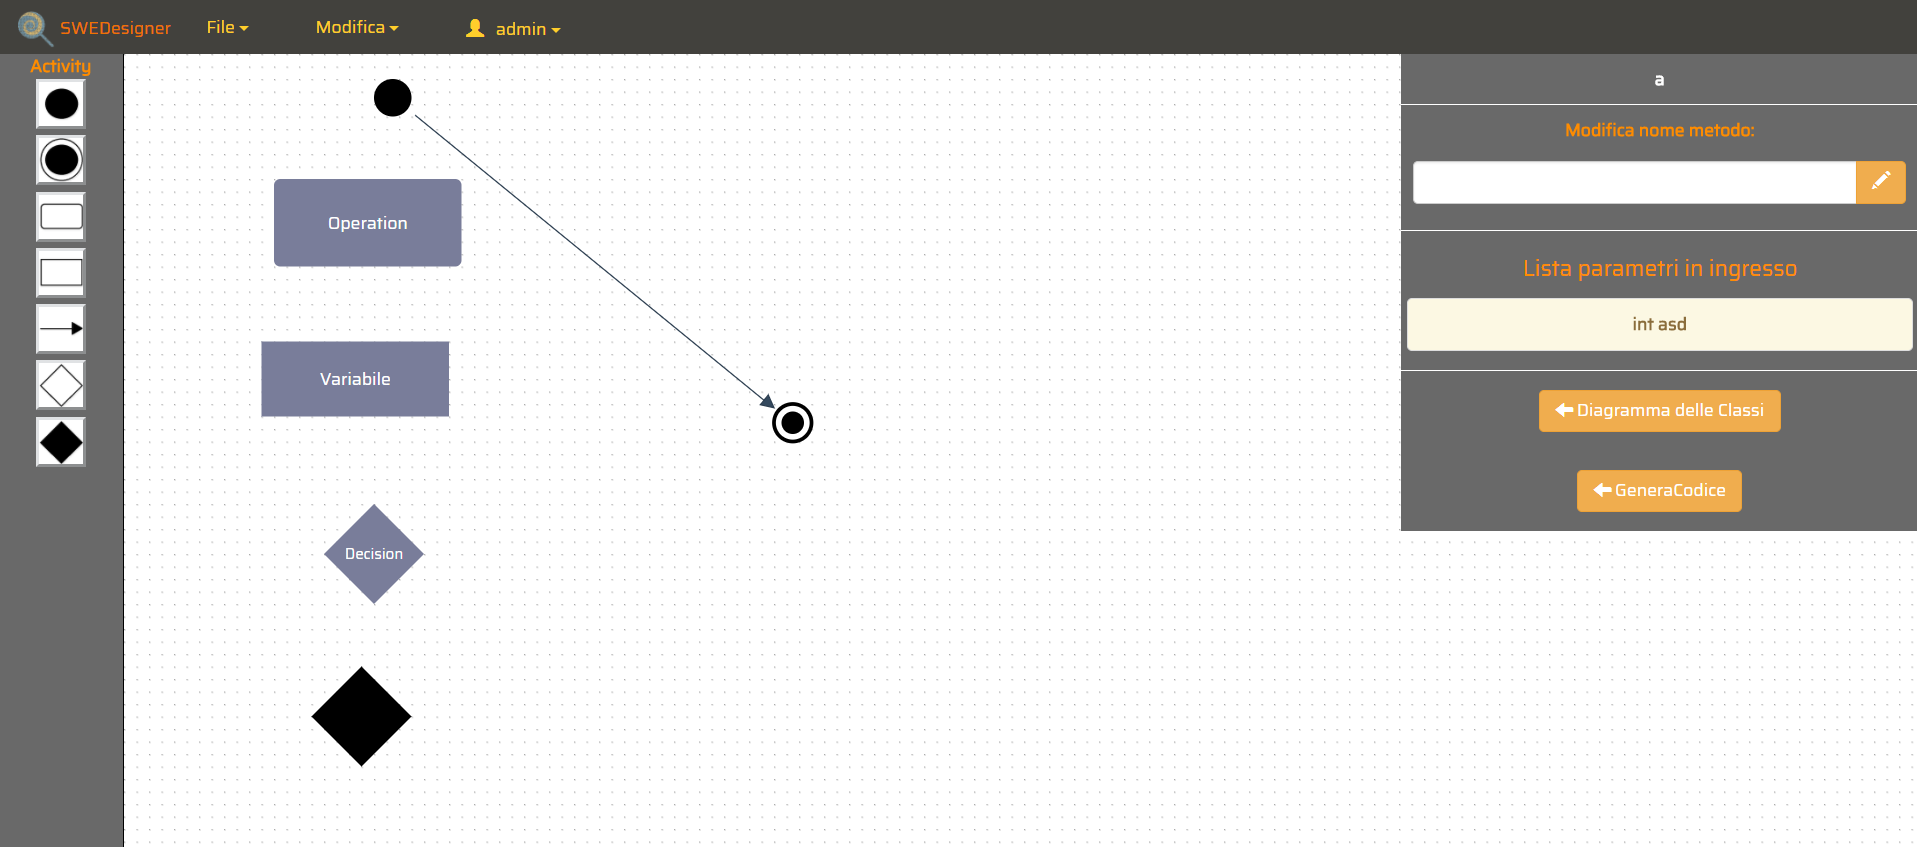
\includegraphics[scale=0.22]{res/img/activity1.png}
		\caption{Editor di un activity}
	\end{figure}
	In questa sezione verranno presentati le funzionalità di editing di un metodo attraverso il diagramma delle attività.\\
	Si accede a questa sezione dell'editor premendo sul bottone di modifica di un metodo all'interno dell'editor del diagramma delle classi.\\

	\subsection{Medù di modifica elementi}
	 Per quel che riguarda il nodo di inizio, quello di fine e il nodo di chiusura di una decisione sono disponibili solo le funzionalità di eliminazione della forma disegnata accessibile mediante un click sulla forma
	 e uno sul pulsante \emph{Elimina forma}.\\
	 \subsubsection{Modifica operazione}
		 \begin{figure}[h!]
	 		\centering
	 			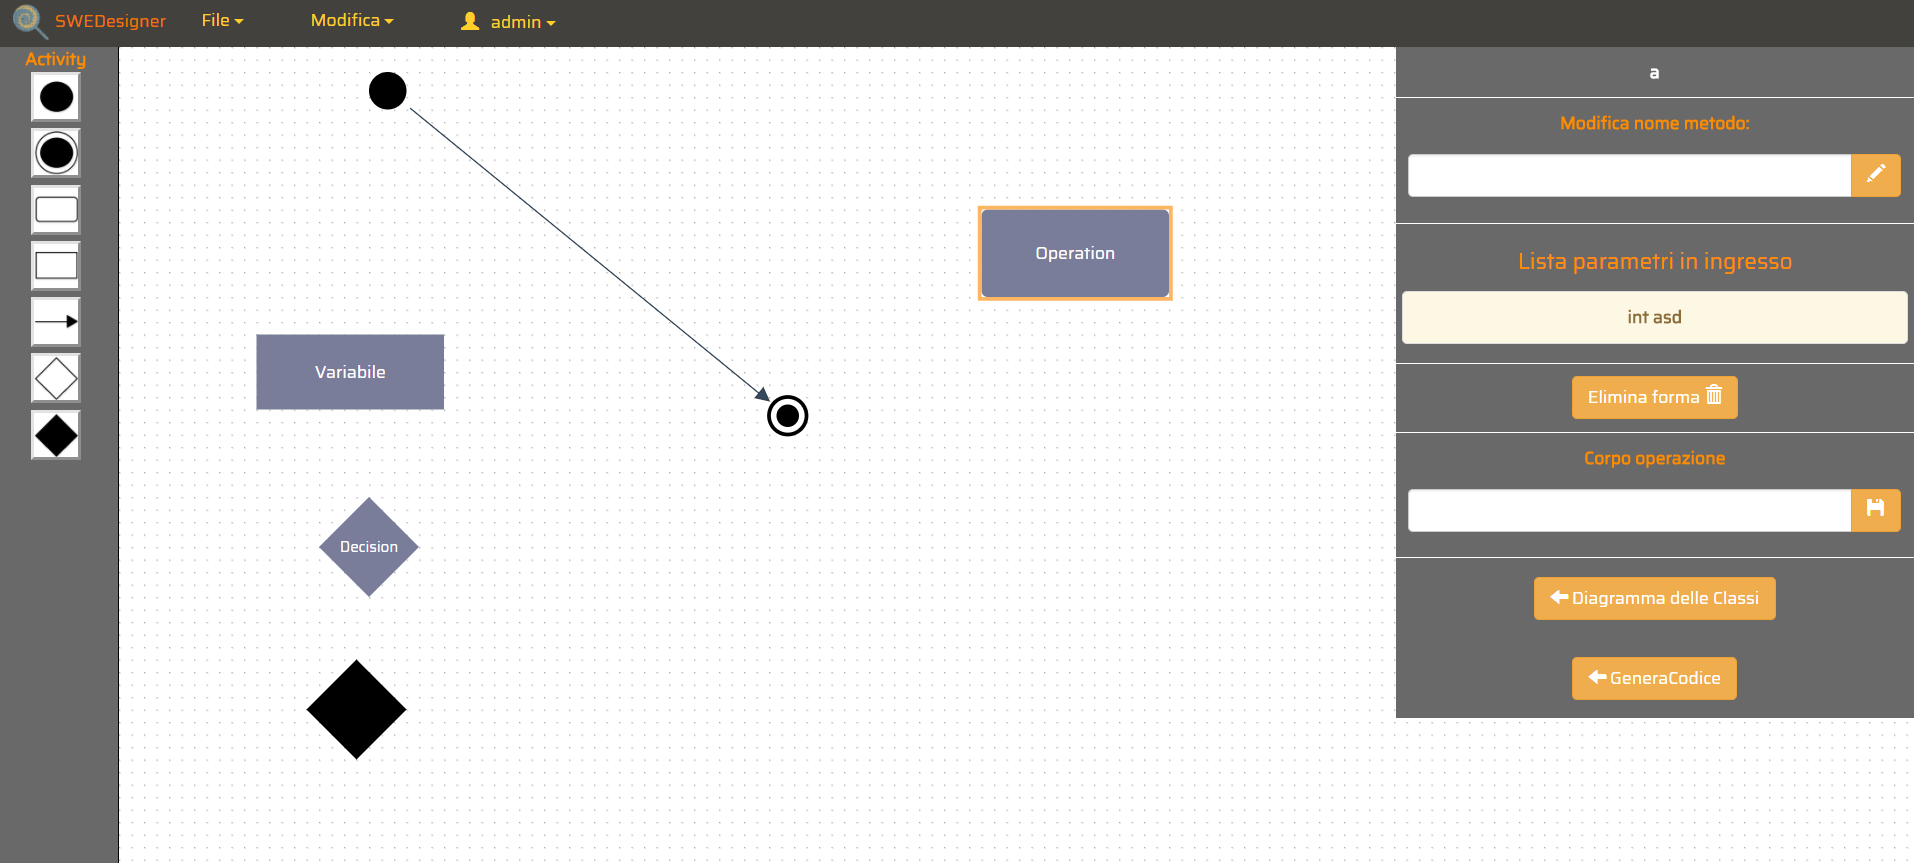
\includegraphics[scale=0.22]{res/img/activity2.png}
	 		\caption{Editor di un'operazione}
	 	\end{figure}
		In questa sezione è possibile modificare un'operazione scrivendo a mano, all'interno dell'input \emph{Corpo operazione}, il corpo dell'operazione che è possibile
		aggiungere mediante un click sull'icona di salvataggio.
	\subsubsection{Modifica variabile}
		\begin{figure}[h!]
		 \centering
			 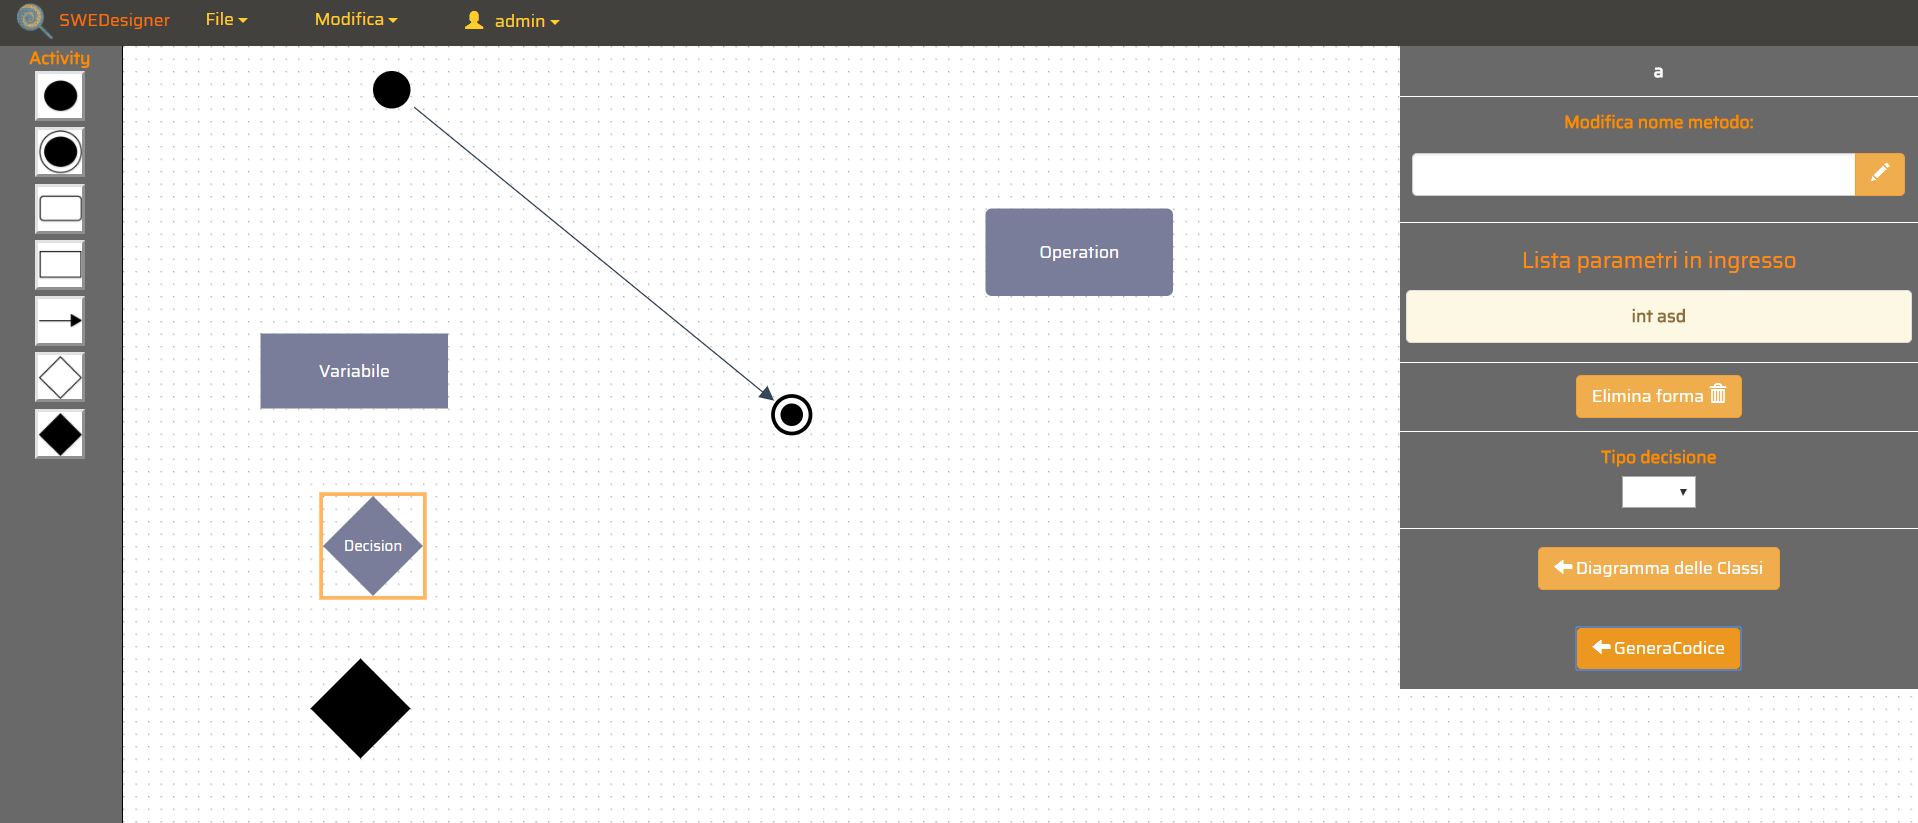
\includegraphics[scale=0.22]{res/img/activity3.png}
		 \caption{Editor di una variabile}
	 \end{figure}
		In questa sezione è possibile modificare una variabile inserendone nome, tipologia e valore.\\
		È possibile utilizzare sia la modalità guidata, che guida passo passo l'utente, o passare alla modalità libera mediante un click su \emph{cambia modalità} che consente di scrivere
		codice liberamente.\\
	\subsubsection{Modifica decisione}
		\begin{figure}[h!]
		 \centering
			 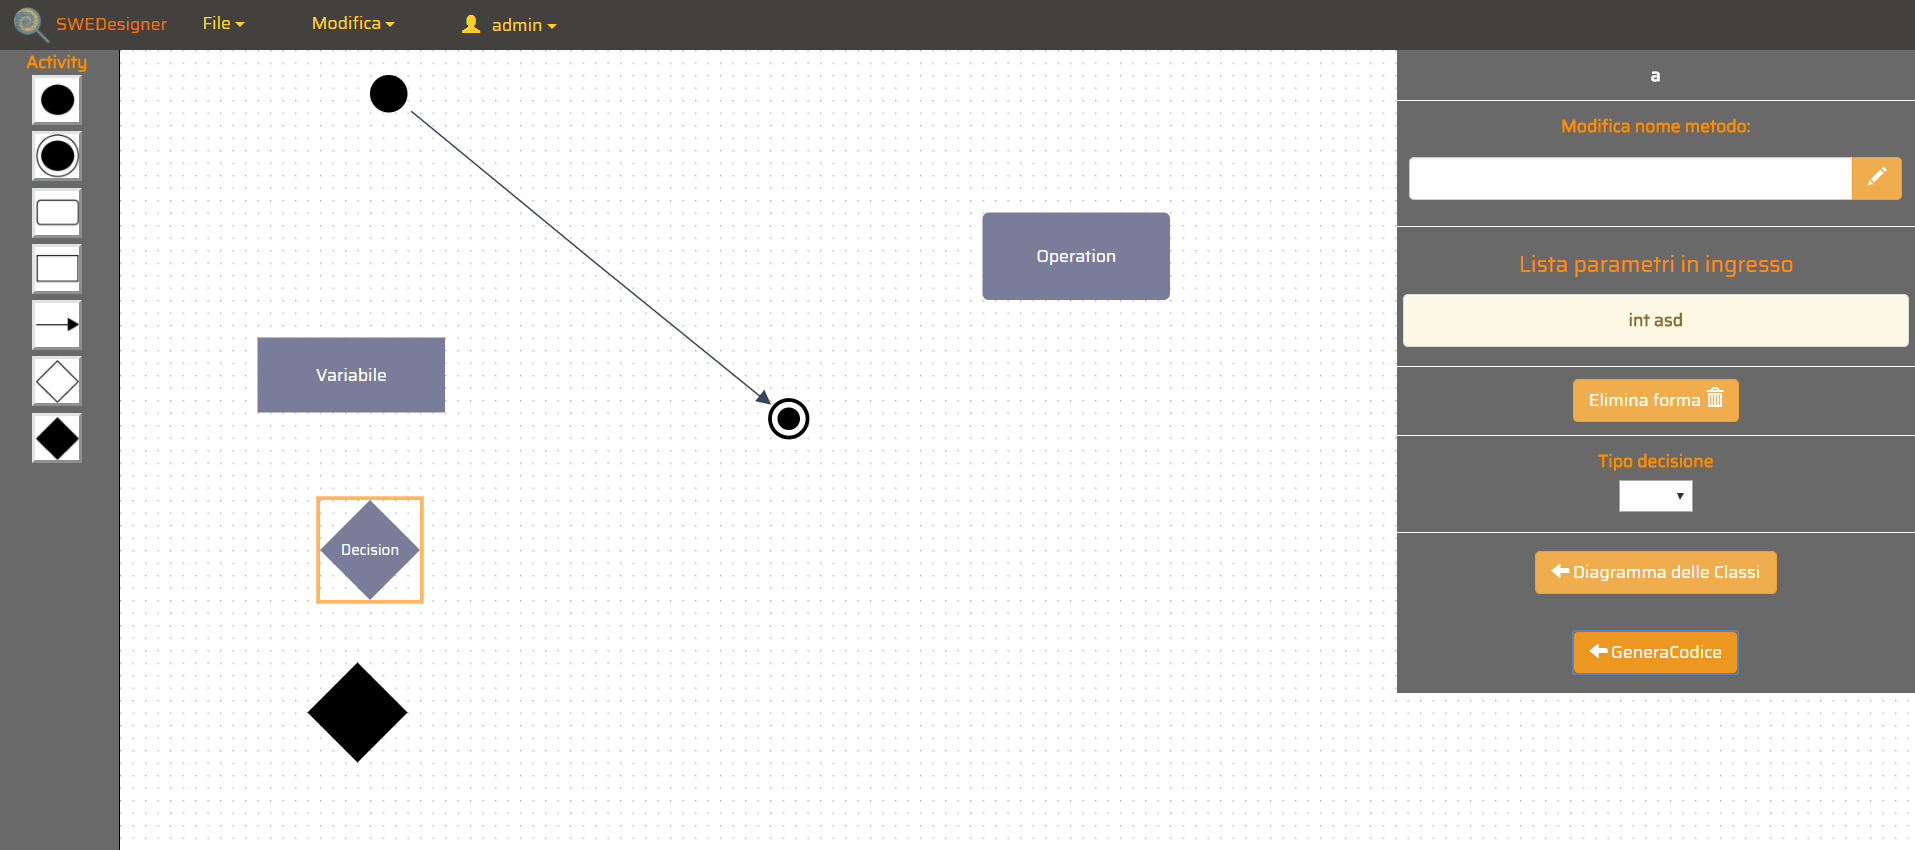
\includegraphics[scale=0.22]{res/img/activity4.png}
		 \caption{Editor di una decisione}
	 \end{figure}
	 In questa sezione è possibile modificare una decisione scegliendone il tipo, if, for o while.\\
 	È possibile utilizzare sia la modalità guidata, che guida passo passo l'utente, o passare alla modalità libera mediante un click su \emph{cambia modalità} che consente di scrivere
 	codice liberamente.\\
